\documentclass[runningheads,a4paper]{llncs}

\usepackage[utf8]{inputenc}
\usepackage{graphicx}
\usepackage{listings, color}
\usepackage[bookmarks,bookmarksopen,bookmarksdepth=2]{hyperref}

\graphicspath{ {./img/} }

%% CUSTOM BINDINGS %%

%\usepackage{amsmath}

 
\usepackage{alltt}
\newcommand{\TODO}[1]{\begin{alltt}\textcolor{magenta}{TODO: #1}\end{alltt}}

\newenvironment{LGContent}
{ \par\color{blue} \it \small }
{ \par }

\usepackage{verbatim}
% Use this to hide text in TODO commands and LGContent environments.
%\renewcommand{\TODO}[1]{}
%\renewenvironment{LGContent}{ \comment  }{ }
\newenvironment{LGContent-Hidden}{ \comment  }{ }

\usepackage{xspace}
\newcommand{\om}{[...]\xspace} % omission

\authorrunning{H. Hartmann, T. Wambach, M. Meffert, R. Grimm}

%% END CUSTOM BINDINGS %%

\begin{document}

%============================================================

\title{A Privacy Aware Mobile Sensor Application}

\author{Heinrich Hartmann \and Tim Wambach \and Maximilian Meffert \and R\"udiger Grimm}
\institute{University of Koblenz-Landau}
\maketitle

%============================================================

\begin{abstract}
In this article we analyze the privacy aspects of a mobile sensor
application used for recording urban travel patterns as part of a
travel-survey service. This service has been developed and
field-tested within the Live+Gov EU Project \cite{LiveGov:Prog}. The privacy analysis
follows a structured approach established in
\cite{Grimm:ItSecRefModel}. Eight privacy recommendations are derived,
and have already led to corresponding enhancements of the
travel-survey service.

\keywords{
privacy protection, IT security analysis, sensor data, mobile phones, traffic survey
}

\end{abstract}

%============================================================

\section{Introduction}
\label{sec:intro}


The rise of mobile smart-phones equipped with a wide range of sensors
and the abundance mobile Internet connectivity has paved the way to a
whole new generation of mobile services which ease the daily life of
citizens using them. Apps like Google
Maps\footnote{\url{http://www.google.com/mobile/maps/}} allows the user to
navigate effectively in unknown cities; others track sports activities
in order to optimize training plans or engage in virtual competitions.

Besides the immediate benefits these services reveal a wealth of
private information about the citizen that capture a very detailed
picture of his life. For instance, GPS location tracking can be used
to infer shopping habits or associations with political groups (when
meetings are attended) and accelerometer data can be used to detect
medical conditions like walking disabilities. All this data is highly
sensitive to the citizen's privacy and can be used against the citizen 
if it falls into the wrong hands.

Providers of these new services are faced with a fundamental trade-off
between features and convenience of the service and the protection of
the citizen's privacy. The service has to collect enough data to
support the basic service promises. If too much data is collected the
privacy of the citizen is put at risk, with immediate implications for
the customer trust relation and the acceptance of the service. Also,
leaks of private data can jeopardize the whole business.

In this article we study the privacy risks of a travel-survey service
for urban mobility that is further specified in section \ref{sec:ScenarioDescription}. In section \ref{sec:privacydef} below, we will explain our view on privacy. In order to find the right user control functions we will perform a systematic privacy analysis of our sensor data storage and mining infrastructure following the reference model of IT security analysis \cite{Grimm:ItSecRefModel} in section \ref{sec:privacyanalysis} below.

%============================================================

\section{Scenario Description: Mobile Traffic Survey}
\label{sec:ScenarioDescription}

Travel surveys are regularly conducted by transport authorities which provide
a public transportation infrastructure. With these surveys the current
usage of the public transportation system is assessed and the insights
are used for future planning of bus, tram and subway lines, etc.  For
each survey a large number of citizens (e.g. 5000) is asked to keep
track of their travel patterns for a constraint period of time
(e.g. one month). Traditionally the travel patterns have been recorded
manually in the form of travel diaries. Modern smart-phones are
equipped with a wide range of sensors (in particular GPS) that allow
the recording of travel-patterns in a fully automated way.

The travel services need the personal mobile data for two reasons: firstly, they want to serve their customers individually, for example by guiding them to proximity stations, to recommend adequate travel connections, to inform about delays, or to sell electronic tickets. For this purpose, the personal data for evaluation are related to the individual customers. Secondly, the travel services want to enhance their system, in that they evaluate the demand of stations, connections, changes, ways and time spent by their customers. For this purpose, personal data are anonymized before evaluation.

Within the Live+Gov EU project \cite{LiveGov:Prog}, we have established a first
prototypical implementation of such an automated travel-survey
service. In this section we give a high level description of the
generic service architecture. This description along with the
introduced terminology will serve as a basis for our privacy analysis.

There are three stakeholders involved in the travel-survey service:
The \emph{citizen}, the \emph{service provider} and the \emph{transport
  authority}. The service provider is the operator of all IT systems and
offers the travel-survey service to the transport authority. Figure
\ref{figure:Live+Gov Vulnerabilities} in section \ref{subsubsection:Conflicts of Interests} below contains a schematic
visualization of the relation between these stakeholders.

The \emph{citizen} is a volunteer who is willing to share his personal travel
patterns within the travel-survey event.  He carries a mobile
smart-phone which runs the \emph{sensor collector application}. The
application collects data from various sensors available on modern
smart-phones. In particular accelerometer- and GPS-samples are
collected. Based on the accelerometer data, the application extracts
human activities (e.g. running, walking, standing). Also, the
application can send raw-sensor data back to a central data center.

The \emph{data center} is under the control of the service provider. It 
stores and processes sensor data collected with
the sensor collector application. It can also take into account data
obtained from third parties, like the current positions of trains. In
particular, the data center determines if the citizen is using public
transportation and if so which lines of service (bus, train, tram) are
used. The data center can also send mining end products and messages
(e.g. traffic jam reports, bus schedule) back to the mobile device of
the citizen.

The \emph{service provider} provides and operates all technical
infrastructure like the data center and the sensor application. He
also operates a web-based \emph{reporting tool} that aggregates
information about travel patterns of citizens within the
travel-survey. The reporting tool is used by the \emph{transport authority} to gain
insights for planning and accounting of the public transportation
infrastructure.





%============================================================

\section{Definition of Privacy}
\label{sec:privacydef}


\subsection{Privacy and Self Data Protection}
1890, the American politician Louis Brandis had specified privacy as the right to be left alone \cite{WarrenBrandeis:RightToPrivacy}. From the data processing point of view, this right is best expressed by the absence of information about a person in the mind of others. Indeed, this principle of “data minimization” is still fundamental to modern data protection legislation. The modern principles of data protection are codified by many legal systems in different countries, especially in Europe \cite{EU-directive2}, and by the US save harbor principles. However, modern data protection is more than only the absence of personal data. It is based on the personal right on self-determination over information and communication \cite{BVerfG:census}. This is, for example, very well expressed by Fried’s definition of 1970:
\begin{quote}
	Privacy is not simply an absence of information about us in the minds of others; rather it is the control we have over information about ourselves. \cite{CFried:Privacy}
\end{quote}
In order to realize this requirement in the modern IT world users are provided with user control functions, for example to decide about the access on their data for future use, and to view, modify, and delete unwanted data that had been collected. In its fundamental decision of May 13, 2014, the European Court has convicted Google to accept user demands to delete links to incorrect or irrelevant personal data in the Internet (C-131/12 – Google Spain SL). Such functions would constitute a so-called self-data-protection. It requires users to be highly aware of their rights and how to use them. Complementary, system-data-protection puts the load of data protection enforcement on the data collectors, ideally even without bothering the users. Typical system data protection functions are the deletion of personal data that are not bound to service purpose, the anonymization of personal data for research, and the abstinence from forwarding personal data to third parties. Together, system-data-protection and self-data-protection are supposed to provide a fair balance between the interests of service providers and their users.
In our research work we focus on self-data-protection according to Fried’s user control requirement \cite{CFried:Privacy}. A system data protection point of view would lead to other results, namely to a set of obligations for service providers. This is subject to further research.


\subsection{The Seven Types of Privacy}
\label{sec:privacytypes}

In Fried's definition of privacy as control over information, the specification of what constitutes such information remains open. There is a vast amount of information that relates to a person and we need to get a better understanding in order to perform a thorough analysis. To this end we use the categorization by Friedewald, Finn and Wright of 2013 called the Seven Types of Privacy \cite{7ToP}. These are an extension to the four types of privacy by Roger Clarke of 1997 \cite{RClarke:4ToP}. It is important to note, that these categories are not mutually exclusive. For instance a written email is considered personal communication as well as personal data stored on a computer. However, the categories are very helpful for a privacy analysis with a focus on self-data-protection.
The seven types of privacy are as follows: Privacy of the Person (with respect to body functions), Privacy of Behavior and Action, Privacy of Communication, Privacy of Data and Image, Privacy of Thoughts and Feelings, Privacy of Location and Space, Privacy of Association (with persons, e.g. friends, and organizations, e.g. political parties).




\subsection{Sensor Data Privacy Impact}
\label{sec:SensorPrivacyImpact}

Modern mobile devices have a broad collection of sensors.
Disclosure or processing of sensor data can impact one's privacy.
In this section we identify groups of sensors and their potential impact on a certain type of privacy.
Figure \ref{figure:Sensor Data Privacy Impact Matrix} qualifies that impact on a simple scale.
Privacy of Data and Image is trivially threatened because here sensor data is individual data, a priori.
Indirect impact is caused by combining sensor data with additional knowledge.
For instance, comparing a contemporary map with locational data can reveal behaviour and thoughts if the position matches a church.

\begin{figure}
\newcommand{\tcell}[1]{\parbox[c][2cm]{4cm}{\vspace{3mm}#1\vspace{3mm}}}
\newcommand{\thead}[1]{\tcell{\Large\centering\textbf{#1}}}
\newcommand{\tbody}[1]{\tcell{\Large\centering #1}}
\centering
\resizebox{\textwidth}{!}{
\begin{tabular}{|c||c|c|c|c|c|c|c|}
\hline
& \thead{Pricacy of the Person}
& \thead{Pricacy of Behaviour and Action}
& \thead{Pricacy of Communication}
& \thead{Pricacy of Data and Image}
& \thead{Pricacy of Thoughts and Feelings}
& \thead{Pricacy of Location and Space}
& \thead{Pricacy of Association}
\\\hline\hline
\thead{GPS Sensor}
& \tbody{0.5} % Pricacy of the Person
& \tbody{0.5} % Pricacy of Behaviour and Action
& \tbody{0} % Pricacy of Communication
& \tbody{1} % Pricacy of Data and Image
& \tbody{0} % Pricacy of Thoughts and Feelings
& \tbody{1} % Pricacy of Location and Space
& \tbody{0.5} % Pricacy of Association
\\\hline
\thead{Motion Sensors}
& \tbody{1} % Pricacy of the Person
& \tbody{0.5} % Pricacy of Behaviour and Action
& \tbody{0} % Pricacy of Communication
& \tbody{1} % Pricacy of Data and Image
& \tbody{0} % Pricacy of Thoughts and Feelings
& \tbody{0} % Pricacy of Location and Space
& \tbody{0} % Pricacy of Association
\\\hline
\thead{Networking Sensors}
& \tbody{0.5} % Pricacy of the Person
& \tbody{0.5} % Pricacy of Behaviour and Action
& \tbody{0} % Pricacy of Communication
& \tbody{1} % Pricacy of Data and Image
& \tbody{0} % Pricacy of Thoughts and Feelings
& \tbody{1} % Pricacy of Location and Space
& \tbody{1} % Pricacy of Association
\\\hline
%\thead{HAR}
%& \tbody{-} % Pricacy of the Person
%& \tbody{-} % Pricacy of Behaviour and Action
%& \tbody{-} % Pricacy of Communication
%& \tbody{-} % Pricacy of Data and Image
%& \tbody{-} % Pricacy of Thoughts and Feelings
%& \tbody{-} % Pricacy of Location and Space
%& \tbody{-} % Pricacy of Association
%\\\hline
%\thead{SLD}
%& \tbody{-} % Pricacy of the Person
%& \tbody{-} % Pricacy of Behaviour and Action
%& \tbody{-} % Pricacy of Communication
%& \tbody{-} % Pricacy of Data and Image
%& \tbody{-} % Pricacy of Thoughts and Feelings
%& \tbody{-} % Pricacy of Location and Space
%& \tbody{-} % Pricacy of Association
%\\\hline
\end{tabular}
}
\newline
\newline
{\scriptsize 
0: No Impact,
0.5: Indirect Impact,
1: Direct Impact}
\caption{Sensor Data Privacy Impact Matrix}
\label{figure:Sensor Data Privacy Impact Matrix}
\end{figure}

\subsubsection{GPS Sensor.}
The GPS sensor gives the current longitude and latitude, the current global position of the mobile device and its carrier, although there is some artificial inaccuracy within civil use. Therefore, the collection of GPS data violates directly the citizens privacy of Location and Space.

%By inference we also get implicit violations of the Privacy of the Person, Privacy of Behavior and Action and Privacy of Association.

\subsubsection{Motion Sensors.}
Accelerometer, Rotation Vector, Gyroscope and Magnetic field sensor measure the physical movement of the mobile device on all three axes.
If the mobile device is carried ``normally'' its safe to say that those sensors also measure the moments of its carrier.
So privacy is infringed regarding biometric behaviour, i.e. the Privacy of the Person.

%By inference we also get implicit violations of the Privacy of Behavior and Action.

\subsubsection{Network Sensors.}
The GSM and WLAN sensors reveal the position of the mobile device and its carrier, when used in connection with external databases (location).
Both sensors give the exact cell or network, the mobile device has registered with at the current moment.
Frequent connection to one particular network also reveals Association, e.g. university networks. The Bluetooth sensors record lists of the bluetooth clients in the direct neighbourhood.
Since those clients are usually moving, inference of the position is usually not possible.
Instead, bluetooth clients carried by a third person may infringe the Privacy of Association.

%A similar argumentat applies to WLAN snsors. 
%If one frequently connects with an organizational wireless network, e.g.~an university network, an association can be deduced (student or staff).

%\subsubsection{Human Activity Recognition.}
%The detection and collection of human activities like walking, standing and running, can interfer with the Privacy of the Person, e.g.~since these movement patterns can be indicators for a person's health. Also, trivially, Privacy of Data and Image is violated.
%
%\subsubsection{Service Line Detection.}
%The detection and collection of the service line the user currently uses in the public transportation system allows inference of the location of the user, at least when entering and leaving those service lines at e.g.~bus stops.
%Implicit privacy violations apply accordingly.


\begin{LGContent-Hidden}

%input{./figures/LG-Implicit-Sensor-Privacy-Matrix}

%TODO: Reformulate the section.
% - Too much overlap with preceeding sections.
% - Structure should be per Sensor Type
% - Add HAR and SLD!

In this section we analyze the impact of the disclosure sensor data and certain processing results to the citizens privacy.
This analyisis builds upon the preceeding analyis, but is more focused on the concrete type of data vailable.
For example, the disclosure of Service Line Detection results, does violate the Privacy of Location and Space but not the Privacy of Association that is violated by general GPS tracking.

\textbf{GPS Data}.
The GPS sensor gives the current longitude and latitude, the current global position of the mobile device and its carrier, although there is some artificial inaccuracy within civil use. Threefore, the collection of GPS data violates directly the citizens privacy of Location and Space, and the privacy of Data an Image.

By inference we also get implicit violations of the Privacy of the Person, Privacy of Behavior and Action and Privacy of Association.

\textbf{Motion Sensors.}
Accelerometer, Rotation Vector, Gyroscope and Magnetic field sensor measure the physical movement of the mobile device on all three axes.
If the mobile device is carried ``normally'' its safe to say that those sensors also measure the moments of its carrier.
So his privacy is infringed regarding biometric behaviour, as it is captured automatically
Privacy of Data and Image is trivially threatened because here sensor data is individual data, a priori.

By inference we also get implicit violations of the Privacy of Behavior and Action.

\textbf{Network Sensors.}
The GSM and WLAN sensors reveal the position of the mobile device and its carrier, when used in connection with external databases.
The GSM sensor gives the exact cell, the mobile device has registered with at the current moment.

The Bluetooth sensors record lists of the bluetooth clients in the direct neighbourhood.
Since those clients are usually moving, inference of the position is usually not possible.
Instead, bluetooth clients carried by a third person may infringe the Privacy of Association.

A similar argumentat applies to WLAN snsors. If one frequently connects with an organizational wireless network, e.g.~an university network, an association can be deduced (student or staff).

\textbf{Human Activity Recognition.}
The detection and collection of human activities like walking, standing and running, can interfer with the Privacy of the Person, e.g.~since these movement patterns can be indicators for a person's health. Also, trivially, Privacy of Data and Image is violated.

\textbf{Service Line Detection.}
The detection and collection of the service line the user currently uses in the public transportation system allows inference of the location of the user, at least when entering and leaving those service lines at e.g.~bus stops.
Implicit privacy violations apply accordingly.

\end{LGContent-Hidden}

%============================================================








\section{Privacy Analysis}
\label{sec:privacyanalysis}

The goal of this chapter is to analyze and identify the threats to personal privacy that are posed by collecting, storing and processing sensor data from mobile phones. We derive concrete privacy protection measures that address the main risks involved with handling such data.

In our analysis we follow the “reference model for IT security analysis” as described in \cite{Grimm:ItSecRefModel}. It supersedes earlier efforts by e.g. \cite{Avizienis}. The reference model consists of a model and a procedure. The model organizes a common security terminology in a reasonable and practical way. The procedure describes a method for analyzing the IT system based on that model. The reference model provides four views: (1) the real world of persons and their assets, (2) the potential world of requirements and threats, (3) measures and plans specified by programs, business models and attack strategies, and, finally, (4) events of running programs, data accesses and performed attacks as well as their defense. In the following sections we apply the proposed procedures of the reference model to our scenario of a travel service that collects personal data from mobile users in order to serve the users and to enhance the service. The service intends to respect the privacy of its users. 

In sections \ref{subsec:world-analysis} and \ref{subsec:pot-analysis} we apply the first two steps of the reference model \cite{Grimm:ItSecRefModel}, which are related to the views on the real world and its privacy risks. In section \ref{subsec:priv-rec} we apply the third step of the reference model by providing specific recommendations and for privacy measures as a result of the previous analysis that the system must comply with. 


\subsection{Step 1. World Analysis}

\label{subsec:world-analysis}

The first step is the \emph{world view} where all components are described in their current state. It consists of the following components: Assets, IT-Systems, Actors, Conflicts of Interests, Vulnerabilities, and Interactions.

The relevant \textbf{IT-Systems} were already described in section \ref{sec:intro}.
\textbf{Interactions} between assets, IT-Systems, humans, and vulnerabilites is partly described in section \ref{sec:intro} and will be further analyzed in section \ref{subsec:pot-analysis}.
	

\subsubsection{Assets}

In this scenario we focus our attention to only one asset: The privacy of the citizen. Our definition of privacy is described in detail in section \ref{sec:privacydef}.

\subsubsection{Actors}
\label{subsubsection:humans}

This section describes the human actors previously introduced in section \ref{sec:ScenarioDescription}. A short description for each actor includes a list of the most important interests.

\textbf{Citizen.}
Citizens are persons who use the mobile device as users of the provided software.
Their main motivation gain convenience in their daily transport activities.
Also they generally benefit from improvements of public infrastructure enabled by data collection.
By using the application, citizens are sharing personal information with the service provider which put their privacy at risk.
Other interests of the citizens include: physical wellbeing and health, financial profit, legitimate use of personal data, non-disclosure of personal data to peers of the citizen, and not being monitored.

\textbf{Malicious External.}
Malicious externals are persons who do not have privileged access to the IT systems, and are willing to break laws, security constrains and norms in order to promote their interests. A common interest of an external is financial profit. For example they want to obtain access to critical systems to steal sensitive data or to get the system under their control. Stolen data could simply be sold as is or used for illegitimate purposes, e.g. spam or phishing attacks - or excessive data mining. In short, externals could be interested in: increase power over citizen, financial profit, political activism, and their social standing.

\textbf{System Provider.}
System providers operate the technical infrastructure (hardware and software) of the IT System. They are private companies and legal persons in their own right, but also employ a number of people with diverging interests including administrators, developers, and support managers. As companies, they are interested in gaining financial profit. 
% The financial success of system providers depends on the task complexity of the maintained infrastructure. 
% The complexity of a task has to be in reasonable bounds, so that system providers can complete it within time, with a satisfying quality.
System providers are interested in: financial profit, limited infrastructure complexity, professional excellence, good working conditions for their employees and good public reputation.

\textbf{Transport Authority.}
Transport authorities are public offices (ministry, agency, department, \dots) or other external public entities which act as direct customers of service providers. For example a department for urban mobility orders a system to better understand usage patterns and make improvement to the urban traffic flow. Such systems are investments, and so naturally transport authorities are interested in a profitable return, like increased ticket sales. Transport authorities are interested in: financial profit, political reputation, business intelligence, and good working conditions.


\subsubsection{Conflicts of Interests}
\label{subsubsection:Conflicts of Interests}
Different actors have different interests which can be in conflict with each other. This section outlines the Conflicts of Interests between the actors of the proposed IT system architecture. The emphasis here is to put on prominent existing conflicts, because they provide a foundation for vulnerabilities and subsequent threats.

\textbf{System Complexity vs Privacy.}
System providers offer a service to transport authorities, so that they are able to improve their public services. This task in it self has a high technical complexity and operates on privacy sensitive data provided by monitored citizens.

\textbf{Business Intelligence vs Privacy.}
Transport authorities are purchasing monitoring and mining services from system providers.
They are naturally interested in gaining as much business intelligence from those services as possible.
This interest is in conflict with the citizens' interest of maintaining control over his data and protecting his privacy.

\textbf{Power of External vs. Privacy.}
Malicious externals which are in a social relation to the citizen can have an interest in obtaining further information in order to gain power. In the most simplistic example this could be a man wanting to monitor the activities of his spouse.

\textbf{Financial Profit of External vs Privacy.}
Malicious Externals can gain financial profit from stealing privacy sensitive data.
For example by selling raw contact information to advertisers or by selling mined data to insurance companies, or intermediaries like scoring companies. In such cases, citizens lose complete control over their data.

\textbf{Financial Profit of External vs Reputation of System Providers.}
Externals have various business models as optional foundation for attacks on system providers.
For instance, they can try to invade the infrastructure for e-espionage reasons, to get control over servers to create a bot network or to steal user data. A successful attack proves the technical competence of system providers wrong and subsequently harms their professional reputation.

\textbf{Political Activism vs Reputation of Transport Authority.}
Besides monetary reasons, externals can be motivated by political reasons to attack the monitoring and mining system.
Externals can break the system to make a political statement of their own,
or they can steal user data to prove the system insecure.
Both would harm the reputation of travel agencies, who endangered the privacy of the citizens.


\subsubsection{Vulnerabilities}
\label{subsubsection:Vulnerabilities}
This section outlines the vulnerabilities of the proposed monitoring and mining system. This is illustrated by figure \ref{figure:Live+Gov Vulnerabilities} below.

%input{./figures/LG-Vulnerabilities}
\begin{figure}
\centering
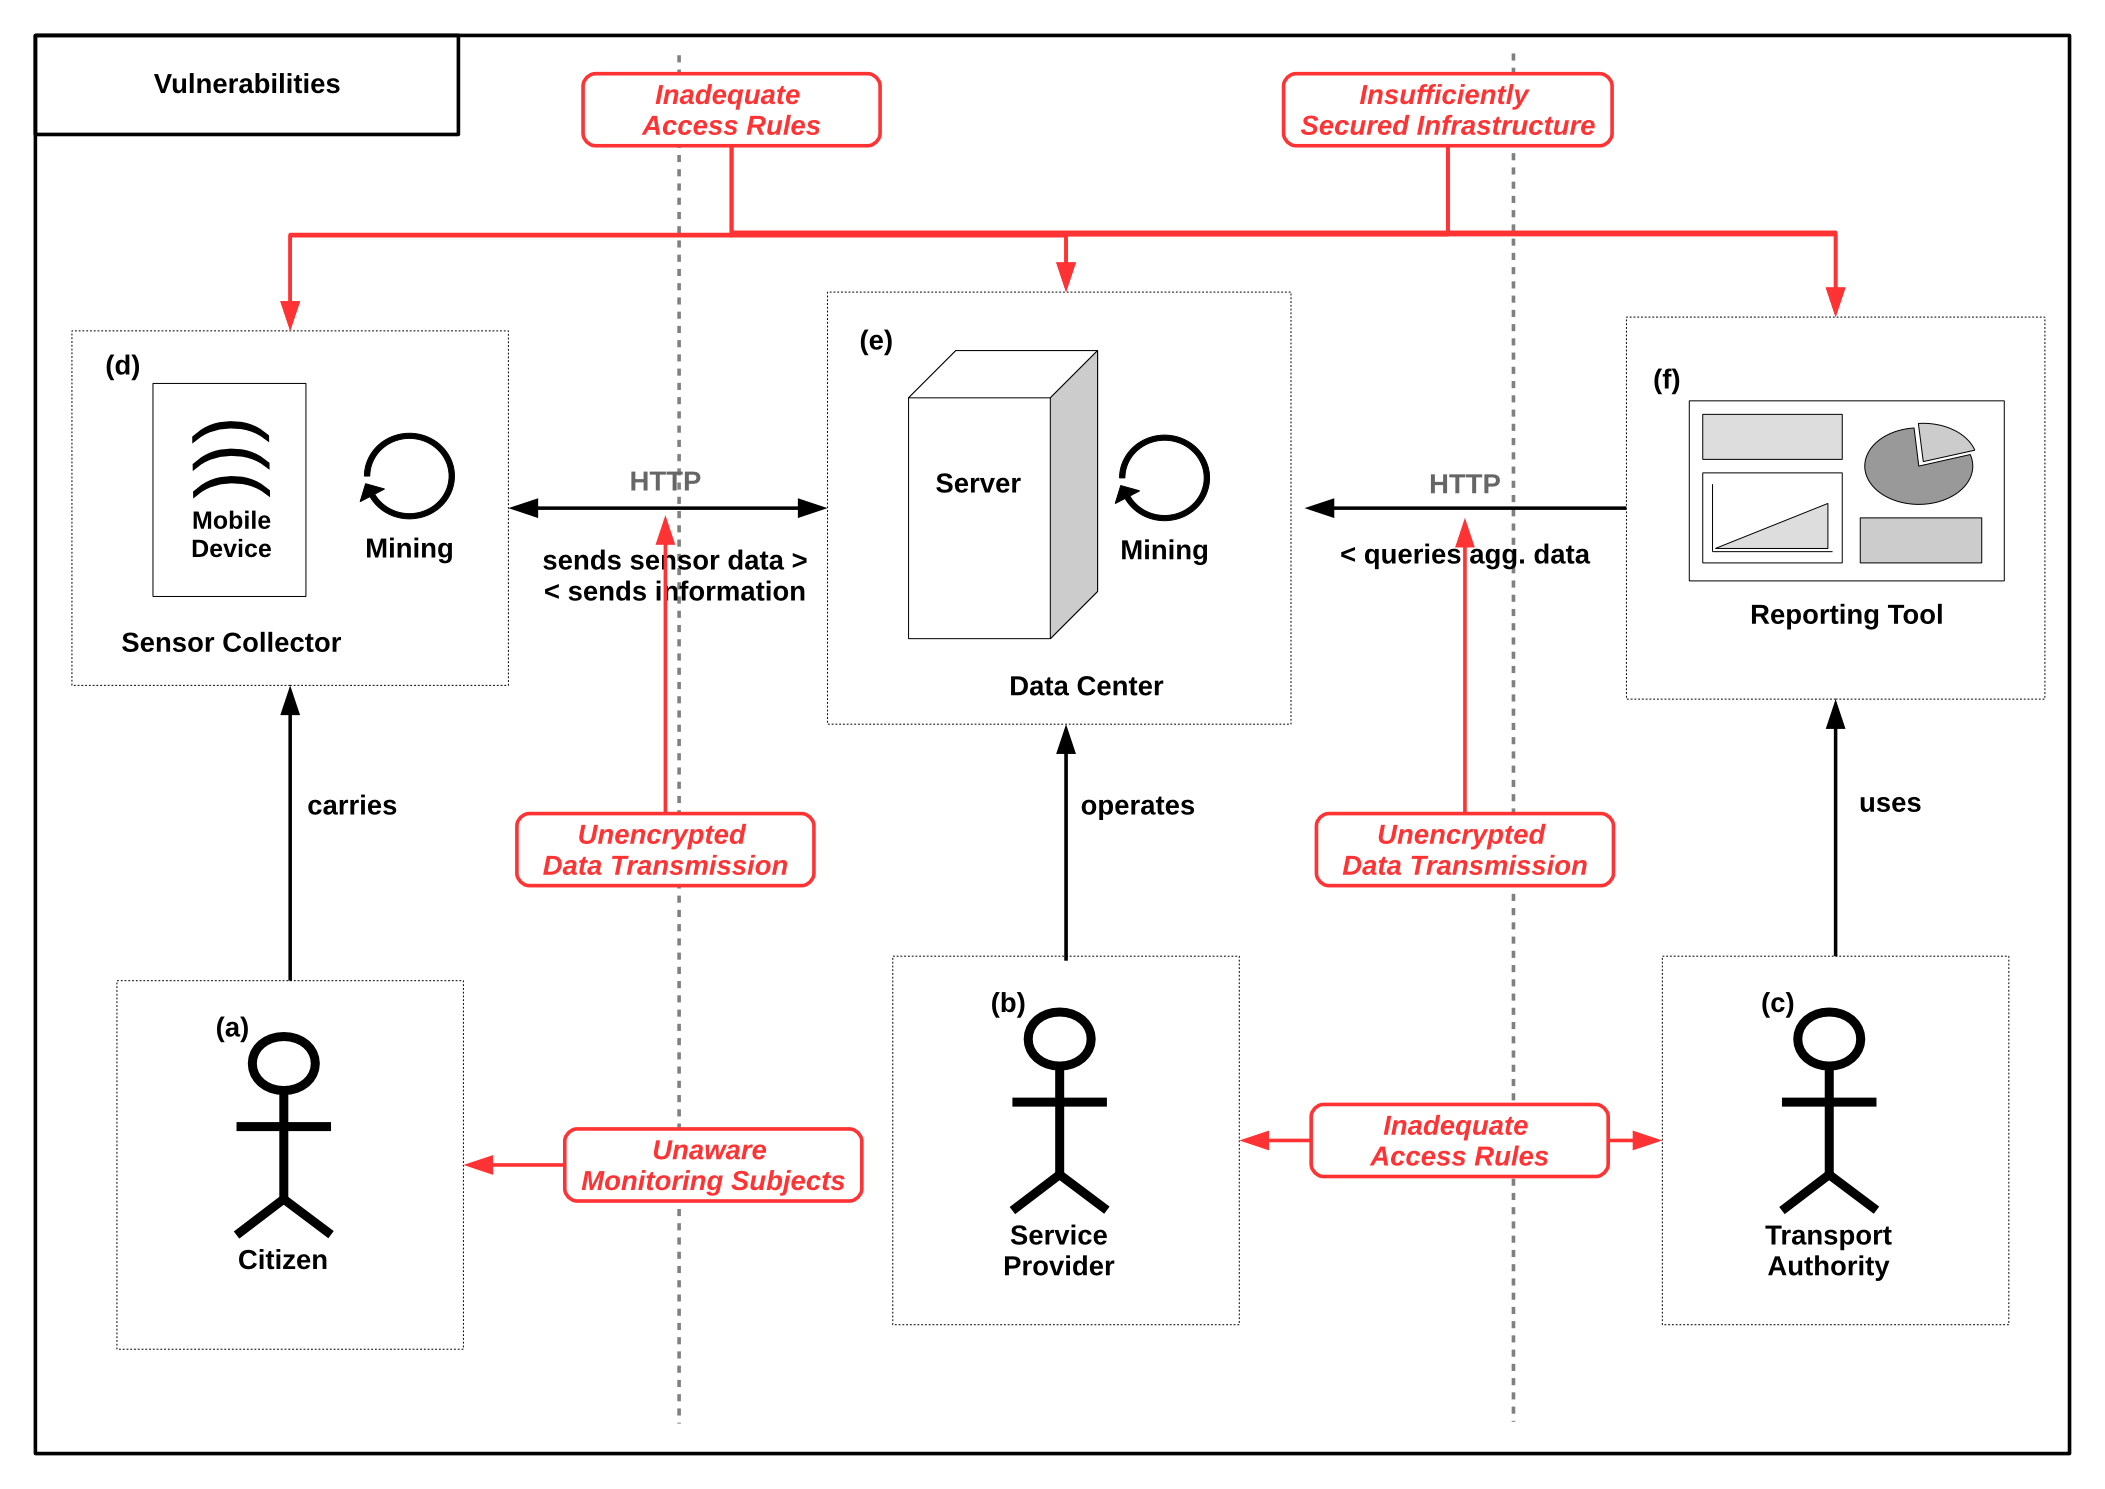
\includegraphics[width=0.6\textwidth]{diagrams/png/vulnerabilities.png}

\caption{Overview of vulnerabilities of the Live+Gov System }
\label{figure:Live+Gov Vulnerabilities}
\end{figure}

\textbf{Insecure Infrastructure.}
The proposed monitoring system consists of many hardware and software components, each with its own concrete weaknesses. For instance, outdated operating systems are frequently vulnerable to attacks.

\textbf{Insecure Data Transmission.}
The proposed monitoring and mining system uses HTTP to exchange data between the sensor collector, the data center and the reporting tool.
Data can be intercept and read all sensitive information, which is send between the components e.g. sensor data and data mining results.

\textbf{Unhappy Employees.}
As an insider, an employee who is frustrated with his situation constitutes a security vulnerability. On the one hand he might
want to harm his employer directly, on the other he is increasingly
susceptible for social engineering.

\textbf{Inadequate Access Rules.}
The proposed IT system infrastructure has various accesses rules for privacy sensitive data.
Administrators of the system provider need full access to data center hardware and software.
Developers and sales managers only have limited access.
Transport authority staff has access to the reporting tool but not to the raw data.
Ill configured or ineffective access systems expose data to non-authorized personal and create a vulnerability.

\textbf{Unaware Monitoring Subjects.}
We define privacy as the ability to control information about oneself. 
In order to do that, monitored subjects need to know, that
they are monitored, who monitors them, what information is recorded
and for what purposes.  Subjects who are not aware of these things
cannot effectively preserve control and thus lose their privacy. 

\subsection{Step 2. Potential World Analysis}
\label{subsec:pot-analysis}

The \emph{Potential World Analysis} displays the intended and unintended interactions of the components in the world view. The intended interactions support the underlying business objectives. Unintended interactions can lead to threats. Obviously this provides a conflict of interest with the victim's business model, to keep the asset away from unauthorized access. From the point of view of the victim, an attack would be an unintended interaction. The potential world view consists of the following components: Business Objectives, Threats, Chances/Risks, and Security Requirements. 
\textbf{Business Objectives} of the system owner were already described in section \ref{sec:intro} and \ref{subsec:world-analysis}. \textbf{Security Requirements} are included to our analysis in section \ref{subsec:priv-rec}.


\subsubsection{Threats}

A threat is a potential interaction of the components that targets an asset.
We restrict ourselves to the case of attacks, and the asset of privacy.
An attack is an interaction that is executed by an actor in response to a conflict of interest by exploiting a vulnerability of the system. We describe threats for the citizen's privacy in the system. As a matter of course, this list cannot be complete, but we make a best effort to cover the most relevant cases.

\textbf{T1. Insufficient Control Features.}
As soon as collected data of citizens is stored on system provider servers all control over that data is lost,
unless features are built into the system that enable citizens to control their data explicitly.
These control features add to the system complexity and require extra effort by the system provider.
Therefore interests of citizens and system providers are in conflict, namely it is the citizen's \textit{Privacy vs. System Complexity} for system providers.

\textbf{T2. Excessive Data Mining.}
The system provider and/or the transport authority secretly extract more private information from the collected data, than the citizen agreed to. This could be the case for a system provider, who wants to test a new product and uses the pre-existing data collection.
Although this mining process do not need to create a direct harm for the citizen (e.g. when there is no disclosure to third parties) the control over his data is lost and thus his privacy is violated. 
There are two conflicts of interest involved: \textit{Privacy vs. Financial Profit of Serivce Provider} and  \textit{Privacy vs. Buisness Intelligence of Transport Authority}.
The threat can be provoked by either careless data handling policies of both system providers and transport authorities, or a weak rule enforcement of existing supervision. But the main issue, which can lead to such threats, is again a general \textit{Missing Privacy Awareness}.

\textbf{T3. Data Theft}
An malicious external infiltrates the infrastructure in order to steal personal data and sell it on the black market. Also the External might be motivated politically and wants to harm the reputation of the system provider or the transport authority. Such a successful attack could harm the reputation of both system provider and transport authority. This threat is defined by three conflicts: \textit{Privacy vs. Financial Profit}, \textit{Reputation of Service Provider vs. Political Activism} and \textit{Reputation of Transport Authority vs. Political Activism}. Also this threat describes the classical scenario, where attacks are provoked by \textit{Insecure Infrastructure} (SQL injection) and \textit{Insecure Communication}.

\textbf{T4. Surveillance}
An External infiltrates infrastructure in order to obtain information
about citizens and exploit it directly.  In this scenario the
external is supposed to have some direct relationship to the citizen
which motivates his interest to obtain personal information.  Examples
could be a public institution that wants to gain information about
planned activities of the citizens (e.g. Nixon's Watergate scandal or
the recent prosecution of Guardian journalists by GHCQ). 
In this threat the privacy interest of the citizen is in conflict with
the aspirations for power over citizens by the externals.

\textbf{T5. Information Leak} 
Like a malicious external person in the data theft scenario an employee of the
service provider or the transport authority has selfish interests to gain
money, make political statements or harm his employer.  In order to
pursue this interest he can steal personal data and sell it or release
it to the public.  The corresponding conflicts of interests are:
\textit{Privacy vs. Financial Profit} of the employee, \textit{Reputation of Service
  Provider vs. Political Activism} of the employee and \textit{Reputation of Transport
  Authority vs. Political Activism} of the employee.  The vulnerability constitutes of
the existence of \textit{Unhappy employees} and possibly \textit{careless access
rules}, which enable the employee to obtain large amounts of data
unnoticed.

\textbf{T6. Social Engineering}
In this scenario an external manipulates an employee of a service
provider or the transport authority to leak information to the external
person.  It is thus a combination of the data theft and Information Leak
scenario.
The conflicts of interest are \textit{Privacy vs. Financial Profit} of
the external, \textit{Reputation of Service Provider vs. Political
  Activism} of the external and \textit{Reputation of Transport Authority
  vs. Political Activism} of the external.  The exploited
vulnerabilities are, again, the existence of \textit{Unhappy
  employees} and possibly \textit{careless access rules} that enable the
employee to obtain large amounts of data unnoticed.

\subsubsection{Chances/Risks}

In this section we will associate to every identified threat with a corresponding risk. A risk is the expected loss that is associated to the threat.
Therefore, we have to quantify the likeliness of the threat to occur and the harm or loss done in this case.
The quantification of likeliness will be solely based on rough judgment of the authors.
The quantification of loss will be made in a two step process.
For each threat listed in the previous section, we have analyzed the affected personal data of the citizen.
For each possible data type (e.g. GPS) we analyze the impact on the seven different types of privacy in section \ref{sec:SensorPrivacyImpact}.
In combination we can quantify roughly the impact of each threat on the citizens privacy. 

For the quantification of the loss in case of a threat scenario we use the following rough calibration between 3 (high) and 0 (none). For the quantification of likeliness the following scale between 4 (always) and 0 (impossible) is used. For the quantification of the risk, we add the values for loss and likeliness of the corresponding threats. Note, that loss and
likeliness scales have a logarithmic character, so that addition
of those scales corresponds to multiplication of the usual scales. The likeliness, loss and the resulting risks assigned to the threats
are discussed in the following paragraphs and summarized in figure
\ref{fig:risks}.

\textbf{Risk of T1. Insufficient Control Features.}  This threat depends on the design of the system. In our case it is always there,
since we do not give the citizen control over his data once it is
recorded. Therefore the Likeliness is evaluated as $4$ (Always).  The
associated, risk is $1$ Low on our scale, since no direct harm is done to
the citizen by exploiting the data. Hence the resulting risk is calculated as $4+1 = 5$.

\textbf{Risk of T2. Excessive Data Mining.}
We assess the likeliness of excessive data mining to be $3$ High, since
this kind of analysis can be performed within the walls of the service
provider, without somebody else noticing, and the service provider himself
has an interest in this activity. The associated loss, on the other hand can be substantial (Medium $2$). Hence the resulting risk is calculated as $3+2 = 5$.

\textbf{Risk of T3. Data Theft.}
The likeliness of a targeted attack by a third party dependens on
the popularity of the offered service and on the financial value of the
captured information. Moreover, the amount of manual work required to
infiltrate a custom build system is significantly higher that that of
compromising a standard software solution. In the scenario we assume a
moderate popularity in a single metropolitan area, with around 10.000
users and storage of data of only limited financial value (no
addresses, no payment information). Therefore the likeliness
assessment is $1-2$ (Low-Medium). The harm of leaked information to a criminal party is $3$ High. Hence the resulting risk is calculated as $4-5$.

\textbf{Risk of T4. Surveillance.}  In the surveillance scenario a party
related to the citizen, like a company that he is customer of, or a
government agency, seeks to obtain sensitive information from our
service. The likeliness of such an intrusion is hard to asses, and depends
again on the popularity of the service. If a high popularity is
reached we have recently learned that spying by government agencies is
very likely to occur. The barrier for companies that do not operate
the infrastructure used to transmit the data a surveillance attack is very 
hard to break. Therefore we assess the likeliness of
the threat with $1-2$ (Low-Medium). The harm of leaked information to a related party is $3$ High. Hence the resulting risk is calculated as $4-5$.

\textbf{Risk of T5/6. Information Leak and Social Engineering.} In our scenario we assume that the culture and ethics inside the
service provider company and travel agencies are very high, so that
the information leak scenario has a likeliness of $1$ (Low). The harm of such an information leaked is $3$ High, so that the
resulting risk is calculated as $4$.


\begin{figure}
\centering
\begin{tabular}{|l|l|l|l|l|}
\hline
\textbf{Threat}                   & \textbf{Likeliness} & \textbf{Loss} & \textbf{Risk} & \textbf{Recommendation}
\\\hline
T1. Insufficient Control Features & 4                   & 1             & 5             & R1, R2
\\\hline
T2. Excessive Data Mining         & 3                   & 2             & 5             & R3, R4, R5
\\\hline
T3. Data Theft                    & 1 - 2               & 3             & 4 - 5         & R6
\\\hline
T4. Surveillance                  & 1 - 2               & 3             & 4 - 5         & R7
\\\hline
T5. Information Leak              & 1                   & 3             & 4             & R8
\\\hline
T6. Social Engineering            & 1                   & 3             & 4             & R8
\\\hline
\end{tabular}
\caption{Live+Gov Risk Evaluation and Recommendations}
\label{fig:risks}
\end{figure}


\subsection{Privacy Recommendations}
\label{subsec:priv-rec}

In this section we derive recommendations or
requirements for a system that addresses these risks. The mapping of these recommendations to the threats is summarized in figure \ref{fig:risks}.

\textbf{R1. Privacy Dashboard}. In order to address the threat with the highest risk, Insufficient Control (T1) of the citizen, we need to give the citizen back the
control over his data inside the system. The most direct way to do
this is to provide a web-based overview which allows the citizen to view, edit and delete all information about his person
that is stored inside the system. 

\textbf{R2. Privacy Policy}. A necessary pre-requirement for effective control of the citizen over his data is information and comprehension of the intended data capturing and processing steps. Therefore a policy that
is easily readable and contains all important information is essential and a legal requirement.

\textbf{R3. Data Handling Guidelines}. The threat with the second largest risk is (T2) Excessive Data Mining.
Contrary to common belief, it is neither legal nor ethical to process
personal data by new methods or for new purposes that were not
stated and explained to the citizen at the time of data
collection. Also the common practice of obtaining far-reaching
permissions from the citizens inside the privacy policy is neither an
ethical or legal solution to the problem. To address this threat awareness about the limitations of data
processors inside the company is a key element. As one mean to
establish such a culture of privacy respect, we recommend to prepare
an guideline intended for internal use that explains the concrete processing steps and purposes that have been permitted by the citizens. 

\textbf{R4. User Permissions}. If further processing should be performed, it is necessary to seek additional permissions from the citizens. A simple email explaining the planned processing steps, and asking for permissions would be enough for this purpose. The permission can be given via an embedded link that shall be followed in order to signal agreement.

\textbf{R5. Anonymization}. An alternative measure to address the risk of excessive data mining is the anonymization of data. When all direct- or indirect
links to the identity of the person are removed, no violation of the
citizen's privacy is caused by arbitrary processing. However, removing all
such links is a challenging tasks, and full anonymity is often not
achieved, cf. \cite{krumm2009}.

\textbf{R6. IT Infrastructure Security}. The protection from threat scenario (T3) Data Theft is a case of
classical IT infrastructure security. The storage and processing infrastructure has
to be secured using firewalls, up-to data software versions and proper
authentication mechanisms.

\textbf{R7. Encryption}. The protection from threat scenario (T4) Surveillance focuses on the
communication channels. They are target of wiretapping attacks by
intermediaries or externals with access to the communication
infrastructure. Strong encryption should be used to make
it harder for externals to read the content of the transmitted data.

\textbf{R8. Relationship}. Threat scenarios (T5) Information Leak and (T6) Social Engineering
target the vulnerability of unhappy employees. Therefore a trustful,
healthy company culture should be maintained.

%\end{LGContent}



%============================================================

\section{Conclusion}

The transport authority has a demand for location-based personal data in order to improve its public services. Our goal was to find a balance between this demand of the transport authority and the privacy of the citizens. In a structured manner we identified all actors and their conflicts of interest. We found potential risks and derived recommendations how to protect the citizen's privacy. A central idea of these recommendations is to give the citizens back the control over their data. For example, this can be done by a privacy dashboard in the hand of every user that shows all his or her personal data stored on the system. The implementation of these privacy recommendations satisfies the above-mentioned demand of both sides in compliance with legal data protection requirements.


\bibliographystyle{splncs}
\bibliography{paper}{}



\end{document}
